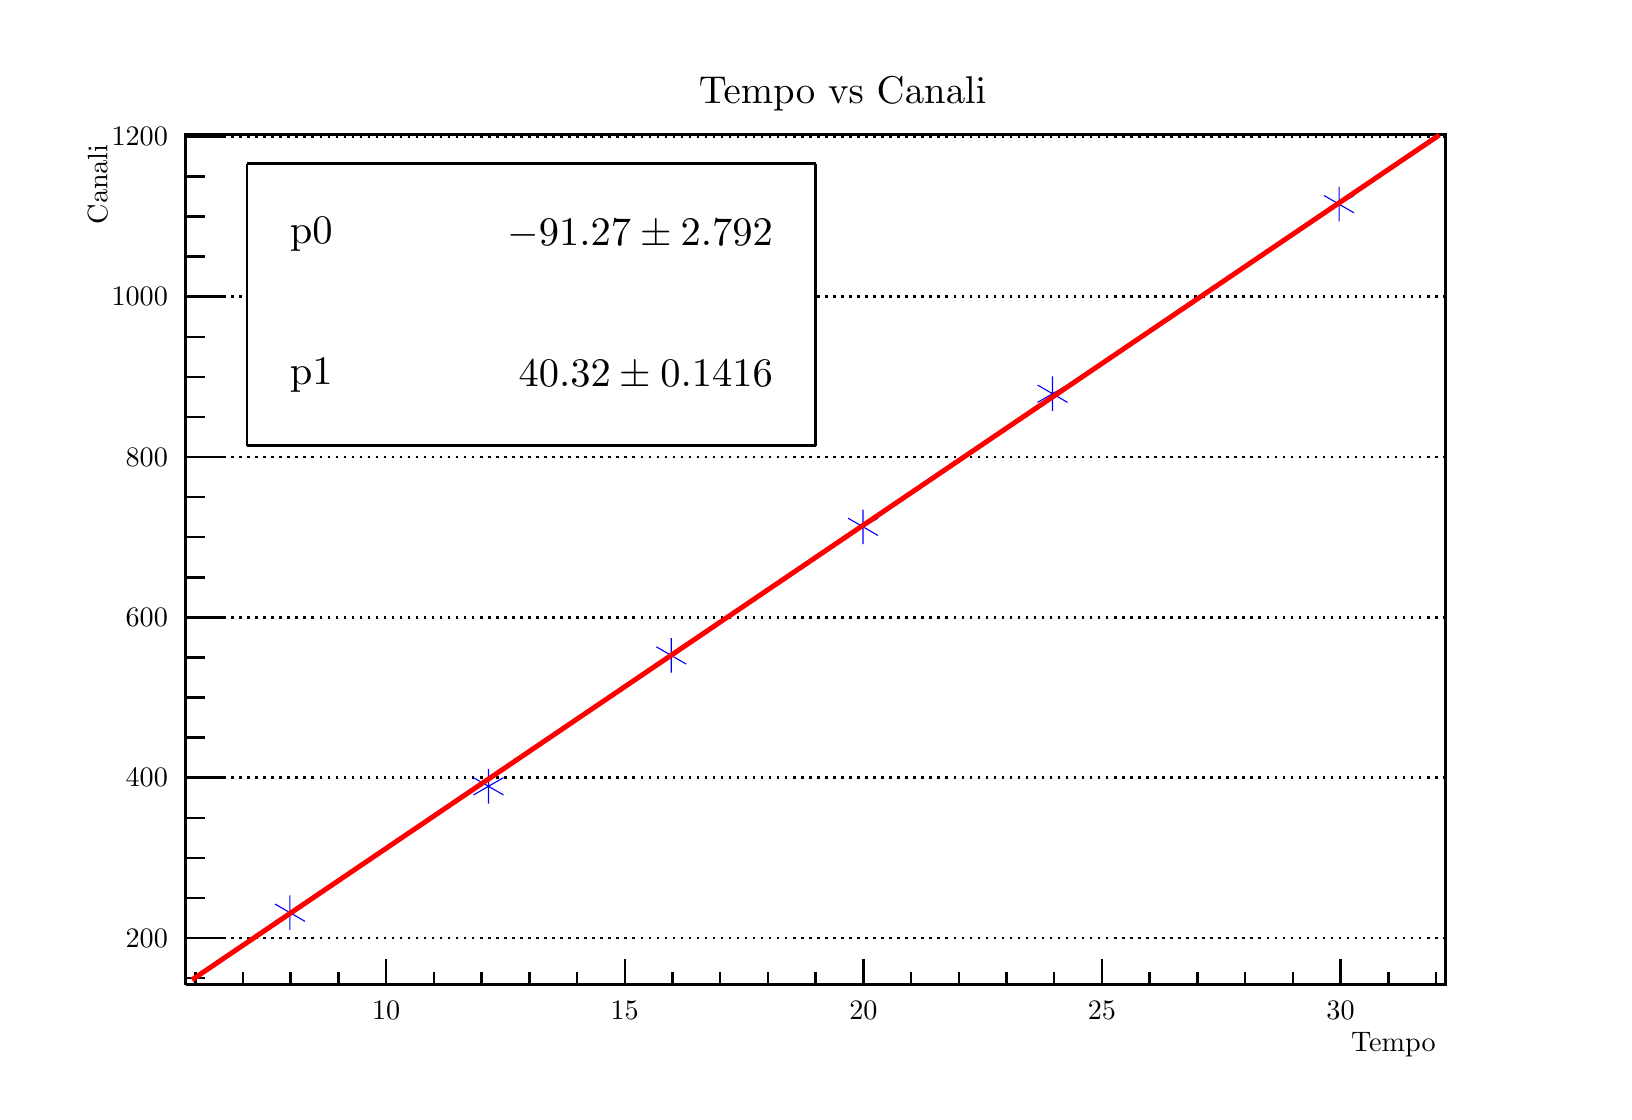
\begin{tikzpicture}
\pgfdeclareplotmark{cross} {
\pgfpathmoveto{\pgfpoint{-0.3\pgfplotmarksize}{\pgfplotmarksize}}
\pgfpathlineto{\pgfpoint{+0.3\pgfplotmarksize}{\pgfplotmarksize}}
\pgfpathlineto{\pgfpoint{+0.3\pgfplotmarksize}{0.3\pgfplotmarksize}}
\pgfpathlineto{\pgfpoint{+1\pgfplotmarksize}{0.3\pgfplotmarksize}}
\pgfpathlineto{\pgfpoint{+1\pgfplotmarksize}{-0.3\pgfplotmarksize}}
\pgfpathlineto{\pgfpoint{+0.3\pgfplotmarksize}{-0.3\pgfplotmarksize}}
\pgfpathlineto{\pgfpoint{+0.3\pgfplotmarksize}{-1.\pgfplotmarksize}}
\pgfpathlineto{\pgfpoint{-0.3\pgfplotmarksize}{-1.\pgfplotmarksize}}
\pgfpathlineto{\pgfpoint{-0.3\pgfplotmarksize}{-0.3\pgfplotmarksize}}
\pgfpathlineto{\pgfpoint{-1.\pgfplotmarksize}{-0.3\pgfplotmarksize}}
\pgfpathlineto{\pgfpoint{-1.\pgfplotmarksize}{0.3\pgfplotmarksize}}
\pgfpathlineto{\pgfpoint{-0.3\pgfplotmarksize}{0.3\pgfplotmarksize}}
\pgfpathclose
\pgfusepathqstroke
}
\pgfdeclareplotmark{cross*} {
\pgfpathmoveto{\pgfpoint{-0.3\pgfplotmarksize}{\pgfplotmarksize}}
\pgfpathlineto{\pgfpoint{+0.3\pgfplotmarksize}{\pgfplotmarksize}}
\pgfpathlineto{\pgfpoint{+0.3\pgfplotmarksize}{0.3\pgfplotmarksize}}
\pgfpathlineto{\pgfpoint{+1\pgfplotmarksize}{0.3\pgfplotmarksize}}
\pgfpathlineto{\pgfpoint{+1\pgfplotmarksize}{-0.3\pgfplotmarksize}}
\pgfpathlineto{\pgfpoint{+0.3\pgfplotmarksize}{-0.3\pgfplotmarksize}}
\pgfpathlineto{\pgfpoint{+0.3\pgfplotmarksize}{-1.\pgfplotmarksize}}
\pgfpathlineto{\pgfpoint{-0.3\pgfplotmarksize}{-1.\pgfplotmarksize}}
\pgfpathlineto{\pgfpoint{-0.3\pgfplotmarksize}{-0.3\pgfplotmarksize}}
\pgfpathlineto{\pgfpoint{-1.\pgfplotmarksize}{-0.3\pgfplotmarksize}}
\pgfpathlineto{\pgfpoint{-1.\pgfplotmarksize}{0.3\pgfplotmarksize}}
\pgfpathlineto{\pgfpoint{-0.3\pgfplotmarksize}{0.3\pgfplotmarksize}}
\pgfpathclose
\pgfusepathqfillstroke
}
\pgfdeclareplotmark{newstar} {
\pgfpathmoveto{\pgfqpoint{0pt}{\pgfplotmarksize}}
\pgfpathlineto{\pgfqpointpolar{44}{0.5\pgfplotmarksize}}
\pgfpathlineto{\pgfqpointpolar{18}{\pgfplotmarksize}}
\pgfpathlineto{\pgfqpointpolar{-20}{0.5\pgfplotmarksize}}
\pgfpathlineto{\pgfqpointpolar{-54}{\pgfplotmarksize}}
\pgfpathlineto{\pgfqpointpolar{-90}{0.5\pgfplotmarksize}}
\pgfpathlineto{\pgfqpointpolar{234}{\pgfplotmarksize}}
\pgfpathlineto{\pgfqpointpolar{198}{0.5\pgfplotmarksize}}
\pgfpathlineto{\pgfqpointpolar{162}{\pgfplotmarksize}}
\pgfpathlineto{\pgfqpointpolar{134}{0.5\pgfplotmarksize}}
\pgfpathclose
\pgfusepathqstroke
}
\pgfdeclareplotmark{newstar*} {
\pgfpathmoveto{\pgfqpoint{0pt}{\pgfplotmarksize}}
\pgfpathlineto{\pgfqpointpolar{44}{0.5\pgfplotmarksize}}
\pgfpathlineto{\pgfqpointpolar{18}{\pgfplotmarksize}}
\pgfpathlineto{\pgfqpointpolar{-20}{0.5\pgfplotmarksize}}
\pgfpathlineto{\pgfqpointpolar{-54}{\pgfplotmarksize}}
\pgfpathlineto{\pgfqpointpolar{-90}{0.5\pgfplotmarksize}}
\pgfpathlineto{\pgfqpointpolar{234}{\pgfplotmarksize}}
\pgfpathlineto{\pgfqpointpolar{198}{0.5\pgfplotmarksize}}
\pgfpathlineto{\pgfqpointpolar{162}{\pgfplotmarksize}}
\pgfpathlineto{\pgfqpointpolar{134}{0.5\pgfplotmarksize}}
\pgfpathclose
\pgfusepathqfillstroke
}
\definecolor{c}{rgb}{1,1,1};
\draw [color=c, fill=c] (0,0) rectangle (20,13.4957);
\draw [color=c, fill=c] (2,1.34957) rectangle (18,12.1461);
\definecolor{c}{rgb}{0,0,0};
\draw [c,line width=0.9] (2,1.34957) -- (2,12.1461) -- (18,12.1461) -- (18,1.34957) -- (2,1.34957);
\definecolor{c}{rgb}{1,1,1};
\draw [color=c, fill=c] (2,1.34957) rectangle (18,12.1461);
\definecolor{c}{rgb}{0,0,0};
\draw [c,line width=0.9] (2,1.34957) -- (2,12.1461) -- (18,12.1461) -- (18,1.34957) -- (2,1.34957);
\draw [c,line width=0.9] (2,1.34957) -- (18,1.34957);
\draw [c,line width=0.9] (2,1.34957) -- (2,12.1461);
\draw [c,dotted,line width=0.9] (18,1.94079) -- (2,1.94079);
\draw [c,dotted,line width=0.9] (18,3.97703) -- (2,3.97703);
\draw [c,dotted,line width=0.9] (18,6.01328) -- (2,6.01328);
\draw [c,dotted,line width=0.9] (18,8.04952) -- (2,8.04952);
\draw [c,dotted,line width=0.9] (18,10.0858) -- (2,10.0858);
\draw [c,dotted,line width=0.9] (18,12.122) -- (2,12.122);
\draw [c,dotted,line width=0.9] (18,1.94079) -- (2,1.94079);
\draw [c,dotted,line width=0.9] (18,12.122) -- (2,12.122);
\draw [c,line width=0.9] (2,1.34957) -- (18,1.34957);
\draw [anchor= east] (18,0.593811) node[scale=1.01821, color=c, rotate=0]{Tempo};
\draw [c,line width=0.9] (4.54545,1.67347) -- (4.54545,1.34957);
\draw [c,line width=0.9] (5.15152,1.51152) -- (5.15152,1.34957);
\draw [c,line width=0.9] (5.75758,1.51152) -- (5.75758,1.34957);
\draw [c,line width=0.9] (6.36364,1.51152) -- (6.36364,1.34957);
\draw [c,line width=0.9] (6.9697,1.51152) -- (6.9697,1.34957);
\draw [c,line width=0.9] (7.57576,1.67347) -- (7.57576,1.34957);
\draw [c,line width=0.9] (8.18182,1.51152) -- (8.18182,1.34957);
\draw [c,line width=0.9] (8.78788,1.51152) -- (8.78788,1.34957);
\draw [c,line width=0.9] (9.39394,1.51152) -- (9.39394,1.34957);
\draw [c,line width=0.9] (10,1.51152) -- (10,1.34957);
\draw [c,line width=0.9] (10.6061,1.67347) -- (10.6061,1.34957);
\draw [c,line width=0.9] (11.2121,1.51152) -- (11.2121,1.34957);
\draw [c,line width=0.9] (11.8182,1.51152) -- (11.8182,1.34957);
\draw [c,line width=0.9] (12.4242,1.51152) -- (12.4242,1.34957);
\draw [c,line width=0.9] (13.0303,1.51152) -- (13.0303,1.34957);
\draw [c,line width=0.9] (13.6364,1.67347) -- (13.6364,1.34957);
\draw [c,line width=0.9] (14.2424,1.51152) -- (14.2424,1.34957);
\draw [c,line width=0.9] (14.8485,1.51152) -- (14.8485,1.34957);
\draw [c,line width=0.9] (15.4545,1.51152) -- (15.4545,1.34957);
\draw [c,line width=0.9] (16.0606,1.51152) -- (16.0606,1.34957);
\draw [c,line width=0.9] (16.6667,1.67347) -- (16.6667,1.34957);
\draw [c,line width=0.9] (4.54545,1.67347) -- (4.54545,1.34957);
\draw [c,line width=0.9] (3.93939,1.51152) -- (3.93939,1.34957);
\draw [c,line width=0.9] (3.33333,1.51152) -- (3.33333,1.34957);
\draw [c,line width=0.9] (2.72727,1.51152) -- (2.72727,1.34957);
\draw [c,line width=0.9] (2.12121,1.51152) -- (2.12121,1.34957);
\draw [c,line width=0.9] (16.6667,1.67347) -- (16.6667,1.34957);
\draw [c,line width=0.9] (17.2727,1.51152) -- (17.2727,1.34957);
\draw [c,line width=0.9] (17.8788,1.51152) -- (17.8788,1.34957);
\draw [anchor=base] (4.54545,0.904212) node[scale=1.01821, color=c, rotate=0]{10};
\draw [anchor=base] (7.57576,0.904212) node[scale=1.01821, color=c, rotate=0]{15};
\draw [anchor=base] (10.6061,0.904212) node[scale=1.01821, color=c, rotate=0]{20};
\draw [anchor=base] (13.6364,0.904212) node[scale=1.01821, color=c, rotate=0]{25};
\draw [anchor=base] (16.6667,0.904212) node[scale=1.01821, color=c, rotate=0]{30};
\draw [c,line width=0.9] (2,1.34957) -- (2,12.1461);
\draw [anchor= east] (0.88,12.1461) node[scale=1.01821, color=c, rotate=90]{Canali};
\draw [c,line width=0.9] (2.48,1.94079) -- (2,1.94079);
\draw [c,line width=0.9] (2.24,2.44985) -- (2,2.44985);
\draw [c,line width=0.9] (2.24,2.95891) -- (2,2.95891);
\draw [c,line width=0.9] (2.24,3.46797) -- (2,3.46797);
\draw [c,line width=0.9] (2.48,3.97703) -- (2,3.97703);
\draw [c,line width=0.9] (2.24,4.4861) -- (2,4.4861);
\draw [c,line width=0.9] (2.24,4.99516) -- (2,4.99516);
\draw [c,line width=0.9] (2.24,5.50422) -- (2,5.50422);
\draw [c,line width=0.9] (2.48,6.01328) -- (2,6.01328);
\draw [c,line width=0.9] (2.24,6.52234) -- (2,6.52234);
\draw [c,line width=0.9] (2.24,7.0314) -- (2,7.0314);
\draw [c,line width=0.9] (2.24,7.54046) -- (2,7.54046);
\draw [c,line width=0.9] (2.48,8.04952) -- (2,8.04952);
\draw [c,line width=0.9] (2.24,8.55858) -- (2,8.55858);
\draw [c,line width=0.9] (2.24,9.06764) -- (2,9.06764);
\draw [c,line width=0.9] (2.24,9.5767) -- (2,9.5767);
\draw [c,line width=0.9] (2.48,10.0858) -- (2,10.0858);
\draw [c,line width=0.9] (2.24,10.5948) -- (2,10.5948);
\draw [c,line width=0.9] (2.24,11.1039) -- (2,11.1039);
\draw [c,line width=0.9] (2.24,11.6129) -- (2,11.6129);
\draw [c,line width=0.9] (2.48,12.122) -- (2,12.122);
\draw [c,line width=0.9] (2.48,1.94079) -- (2,1.94079);
\draw [c,line width=0.9] (2.24,1.43173) -- (2,1.43173);
\draw [c,line width=0.9] (2.48,12.122) -- (2,12.122);
\draw [anchor= east] (1.9,1.94079) node[scale=1.01821, color=c, rotate=0]{200};
\draw [anchor= east] (1.9,3.97703) node[scale=1.01821, color=c, rotate=0]{400};
\draw [anchor= east] (1.9,6.01328) node[scale=1.01821, color=c, rotate=0]{600};
\draw [anchor= east] (1.9,8.04952) node[scale=1.01821, color=c, rotate=0]{800};
\draw [anchor= east] (1.9,10.0858) node[scale=1.01821, color=c, rotate=0]{1000};
\draw [anchor= east] (1.9,12.122) node[scale=1.01821, color=c, rotate=0]{1200};
\definecolor{c}{rgb}{1,1,1};
\draw [color=c, fill=c] (2.77937,8.19484) rectangle (10,11.7765);
\definecolor{c}{rgb}{0,0,0};
\draw [c,line width=0.9] (2.77937,8.19484) -- (10,8.19484);
\draw [c,line width=0.9] (10,8.19484) -- (10,11.7765);
\draw [c,line width=0.9] (10,11.7765) -- (2.77937,11.7765);
\draw [c,line width=0.9] (2.77937,11.7765) -- (2.77937,8.19484);
\draw [anchor= west] (3.1404,10.8811) node[scale=1.46368, color=c, rotate=0]{p0       };
\draw [anchor= east] (9.63897,10.8811) node[scale=1.46368, color=c, rotate=0]{$ -91.27 \pm 2.792$};
\draw [anchor= west] (3.1404,9.09026) node[scale=1.46368, color=c, rotate=0]{p1       };
\draw [anchor= east] (9.63897,9.09026) node[scale=1.46368, color=c, rotate=0]{$ 40.32 \pm 0.1416$};
\definecolor{c}{rgb}{0,0,1};
\foreach \P in {(3.32378,2.26361),(5.84527,3.86819),(8.16619,5.53009),(10.6017,7.16332),(13.0086,8.85387),(16.6476,11.2607)}{\draw[mark options={color=c,fill=c},mark size=6.246246pt,mark=asterisk] plot coordinates {\P};}
\definecolor{c}{rgb}{1,0,0};
\draw [c,line width=1.8] (2.08,1.41032) -- (2.24,1.51869) -- (2.4,1.62706) -- (2.56,1.73543) -- (2.72,1.8438) -- (2.88,1.95217) -- (3.04,2.06054) -- (3.2,2.16891) -- (3.36,2.27728) -- (3.52,2.38564) -- (3.68,2.49401) -- (3.84,2.60238) -- (4,2.71075)
 -- (4.16,2.81912) -- (4.32,2.92749) -- (4.48,3.03586) -- (4.64,3.14423) -- (4.8,3.2526) -- (4.96,3.36097) -- (5.12,3.46934) -- (5.28,3.57771) -- (5.44,3.68608) -- (5.6,3.79445) -- (5.76,3.90282) -- (5.92,4.01119) -- (6.08,4.11956) -- (6.24,4.22793)
 -- (6.4,4.3363) -- (6.56,4.44467) -- (6.72,4.55303) -- (6.88,4.6614) -- (7.04,4.76977) -- (7.2,4.87814) -- (7.36,4.98651) -- (7.52,5.09488) -- (7.68,5.20325) -- (7.84,5.31162) -- (8,5.41999) -- (8.16,5.52836) -- (8.32,5.63673) -- (8.48,5.7451) --
 (8.64,5.85347) -- (8.8,5.96184) -- (8.96,6.07021) -- (9.12,6.17858) -- (9.28,6.28695) -- (9.44,6.39532) -- (9.6,6.50369) -- (9.76,6.61206) -- (9.92,6.72042);
\draw [c,line width=1.8] (9.92,6.72042) -- (10.08,6.82879) -- (10.24,6.93716) -- (10.4,7.04553) -- (10.56,7.1539) -- (10.72,7.26227) -- (10.88,7.37064) -- (11.04,7.47901) -- (11.2,7.58738) -- (11.36,7.69575) -- (11.52,7.80412) -- (11.68,7.91249) --
 (11.84,8.02086) -- (12,8.12923) -- (12.16,8.2376) -- (12.32,8.34597) -- (12.48,8.45434) -- (12.64,8.56271) -- (12.8,8.67108) -- (12.96,8.77944) -- (13.12,8.88781) -- (13.28,8.99618) -- (13.44,9.10455) -- (13.6,9.21292) -- (13.76,9.32129) --
 (13.92,9.42966) -- (14.08,9.53803) -- (14.24,9.6464) -- (14.4,9.75477) -- (14.56,9.86314) -- (14.72,9.97151) -- (14.88,10.0799) -- (15.04,10.1882) -- (15.2,10.2966) -- (15.36,10.405) -- (15.52,10.5134) -- (15.68,10.6217) -- (15.84,10.7301) --
 (16,10.8385) -- (16.16,10.9468) -- (16.32,11.0552) -- (16.48,11.1636) -- (16.64,11.2719) -- (16.8,11.3803) -- (16.96,11.4887) -- (17.12,11.5971) -- (17.28,11.7054) -- (17.44,11.8138) -- (17.6,11.9222) -- (17.76,12.0305);
\draw [c,line width=1.8] (17.76,12.0305) -- (17.92,12.1389);
\definecolor{c}{rgb}{1,1,1};
\draw [color=c, fill=c] (2.77937,8.19484) rectangle (10,11.7765);
\definecolor{c}{rgb}{0,0,0};
\draw [c,line width=0.9] (2.77937,8.19484) -- (10,8.19484);
\draw [c,line width=0.9] (10,8.19484) -- (10,11.7765);
\draw [c,line width=0.9] (10,11.7765) -- (2.77937,11.7765);
\draw [c,line width=0.9] (2.77937,11.7765) -- (2.77937,8.19484);
\draw [anchor= west] (3.1404,10.8811) node[scale=1.46368, color=c, rotate=0]{p0       };
\draw [anchor= east] (9.63897,10.8811) node[scale=1.46368, color=c, rotate=0]{$ -91.27 \pm 2.792$};
\draw [anchor= west] (3.1404,9.09026) node[scale=1.46368, color=c, rotate=0]{p1       };
\draw [anchor= east] (9.63897,9.09026) node[scale=1.46368, color=c, rotate=0]{$ 40.32 \pm 0.1416$};
\draw (10.3438,12.6648) node[scale=1.40004, color=c, rotate=0]{Tempo vs Canali};
\end{tikzpicture}
